%%%%%%%%%%%%%%%%%%%%%%%%%%%%%%%%%%%%%%%%%%%%%%%%%%%%%%%%%%%%%%%%%%%%%%%%%%%%%%%%%%%%%%%%%%%%%%%%%%%%%%%%%%
%Write by:ShuwenHe
%Date:20230613
%%%%%%%%%%%%%%%%%%%%%%%%%%%%%%%%%%%%%%%%%%%%%%%%%%%%%%%%%%%%%%%%%%%%%%%%%%%%%%%%%%%%%%%%%%%%%%%%%%%%%%%%%%

%%%%%%%%%%%%%%%%%%%%%%%%%%%%%%%%%%%%%%%%%%%%%%%%%%%%%%%%%%%%%%%%%%%%%%%%%%%%%%%%%%%%%%%%%%%%%%%%%%%%%%%%%%
\documentclass[12pt,twiside,a4paper]{ctexbook}
\usepackage[centertags]{amsmath}
\usepackage{amsfonts}
\usepackage{amsthm}
\usepackage{newlfont}
\usepackage{makeidx}
\usepackage{wasysym}
\usepackage{geometry} 
\usepackage{graphics}
\usepackage{slashbox} 
\usepackage{fancyhdr} 
\usepackage[pdftex]{graphicx}
\usepackage{epstopdf}
\usepackage{cite}
\usepackage{listings}
\usepackage[numbers,sort&compress]{natbib}

\setlength\parskip{\baselineskip}
\setcounter{tocdepth}{0}
\setcounter{secnumdepth}{4}
\renewcommand\thesection{\arabic{section}}
\usepackage[pdfstartview=FitH,CJKbookmarks=true,bookmarks,bookmarksnumbered=true,
    colorlinks=true,citecolor=black,linkcolor=black,anchorcolor=green,urlcolor=black]{hyperref}
\usepackage{titlesec}
\titleformat{\chapter}[display]{\normalfont\huge\bfseries\center}{\chaptertitlename}{1pt}{\Huge}
\titleformat{\section}{\normalfont\Large\bfseries}{\thesection}{1em}{}
\titleformat{\subsection}{\normalfont\large\bfseries}{\thesubsection}{1em}{}
\titleformat{\subsubsection}{\normalfont\normalsize\bfseries}{\thesubsubsection}{1em}{}
\titleformat{\paragraph}[runin]{\normalfont\normalsize\bfseries}{\theparagraph}{1em}{}
\titleformat{\subparagraph}[runin]{\normalfont\normalsize\bfseries}{\thesubparagraph}{1em}{}
\titlespacing*{\chapter} {0pt}{10pt}{10pt}
\titlespacing*{\section} {0pt}{0.5ex plus 1ex minus .2ex}{0.3ex plus .2ex}
\titlespacing*{\subsection} {0pt}{0.25ex plus 1ex minus .1ex}{0.5ex plus .1ex}
\titlespacing*{\subsubsection}{0pt}{3.25ex plus 1ex minus .2ex}{1.5ex plus .2ex}
\titlespacing*{\paragraph} {0pt}{3.25ex plus 1ex minus .2ex}{1em}
\titlespacing*{\subparagraph} {\parindent}{3.25ex plus 1ex minus .2ex}{1em}
\numberwithin{chapter}{part}
\geometry{left=2.0cm,right=20mm,top=25mm,bottom=25mm}
\let\cleardoublepage\clearpage
%%%%%%%%%%%%%%%%%%%%%%%%%%%%%%%%%%%%%%%%%%%%%%%%%%%%%%%%%%%%%%%%%%%%%%%%%%%%%%%%%%%%%%%%%%%%%%%%%%%%%%%%%%

%%%%%%%%%%%%%%%%%%%%%%%%%%%%%%%%%%%%%%%%%%%%%%%%%%%%%%%%%%%%%%%%%%%%%%%%%%%%%%%%%%%%%%%%%%%%%%%%%%%%%%%%%%
%mathematics
\usepackage{amssymb}
\usepackage{diagbox}
%%%%%%%%%%%%%%%%%%%%%%%%%%%%%%%%%%%%%%%%%%%%%%%%%%%%%%%%%%%%%%%%%%%%%%%%%%%%%%%%%%%%%%%%%%%%%%%%%%%%%%%%%%

%%%%%%%%%%%%%%%%%%%%%%%%%%%%%%%%%%%%%%%%%%%%%%%%%%%%%%%%%%%%%%%%%%%%%%%%%%%%%%%%%%%%%%%%%%%%%%%%%%%%%%%%%%
%
%%%%%%%%%%%%%%%%%%%%%%%%%%%%%%%%%%%%%%%%%%%%%%%%%%%%%%%%%%%%%%%%%%%%%%%%%%%%%%%%%%%%%%%%%%%%%%%%%%%%%%%%%%

%%%%%%%%%%%%%%%%%%%%%%%%%%%%%%%%%%%%%%%%%%%%%%%%%%%%%%%%%%%%%%%%%%%%%%%%%%%%%%%%%%%%%%%%%%%%%%%%%%%%%%%%%%
%
\usepackage{tipa}
%%%%%%%%%%%%%%%%%%%%%%%%%%%%%%%%%%%%%%%%%%%%%%%%%%%%%%%%%%%%%%%%%%%%%%%%%%%%%%%%%%%%%%%%%%%%%%%%%%%%%%%%%%

%%%%%%%%%%%%%%%%%%%%%%%%%%%%%%%%%%%%%%%%%%%%%%%%%%%%%%%%%%%%%%%%%%%%%%%%%%%%%%%%%%%%%%%%%%%%%%%%%%%%%%%%%%
\begin{document}
%%%%%%%%%%%%%%%%%%%%%%%%%%%%%%%%%%%%%%%%%%%%%%%%%%%%%%%%%%%%%%%%%%%%%%%%%%%%%%%%%%%%%%%%%%%%%%%%%%%%%%%%%%

\author
{
Peking University\\
北京大学\\
ShuwenHe\\
何书文\\
1201220707@pku.edu.cn
}

%%%%%%%%%%%%%%%%%%%%%%%%%%%%%%%%%%%%%%%%%%%%%%%%%%%%%%%%%%%%%%%%%%%%%%%%%%%%%%%%%%%%%%%%%%%%%%%%%%%%%%%%%%
\title{C++基础}
\maketitle
\tableofcontents
\pagestyle{fancy}
%%%%%%%%%%%%%%%%%%%%%%%%%%%%%%%%%%%%%%%%%%%%%%%%%%%%%%%%%%%%%%%%%%%%%%%%%%%%%%%%%%%%%%%%%%%%%%%%%%%%%%%%%%

\lhead{
\includegraphics{shuwenedu.png}}
\rhead{科技特长生升学规划 何校长 电话微信15010729356}
\lfoot{
\includegraphics{pku.png}算法第一人北大何书文}
\rfoot{改变您家孩子命运的老师}
%%%%%%%%%%%%%%%%%%%%%%%%%%%%%%%%%%%%%%%%%%%%%%%%%%%%%%%%%%%%%%%%%%%%%%%%%%%%%%%%%%%%%%%%%%%%%%%%%%%%%%%%%%

%%%%%%%%%%%%%%%%%%%%%%%%%%%%%%%%%%%%%%%%%%%%%%%%%%%%%%%%%%%%%%%%%%%%%%%%%%%%%%%%%%%%%%%%%%%%%%%%%%%%%%%%%%
\chapter{C++基础思维导图}
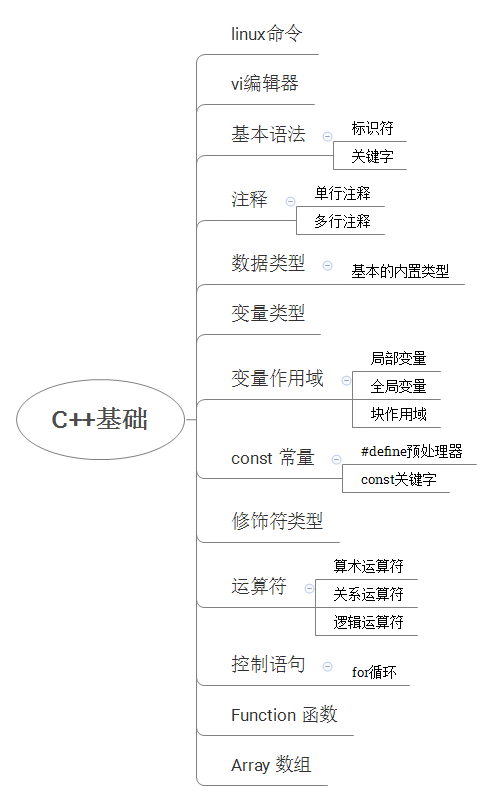
\includegraphics[scale=0.6]{cpp.png}

\chapter{linux命令}
\subsection{文件命令}
mkdir cpp 创建文件夹\\
cd cpp 进入文件夹\\
vi richard.cpp\\
i进入insert模式\\
o进入下一行\\
int 整型\\
main()主函数function\\
// 单行注释\\
“”输入字符串\\
endl\\
;一行语句结束需要用分号结束\\
return 0 一个函数正确执行完成之后需要用return 0来结束\\
esc推出vi编辑器\\
:wq保存并推出 write quit\\
ls查看当前文件夹有什么文件ls - list directory contents

\section{文本编辑器}

\section{C++编译器}
命令行使用下面的命令来检查您的系统上是否安装了gcc\\
g++ -v
g++ 编译器C++\\
使用 -o 选项指定可执行程序的文件名\\
g++ hello.cpp -o hello\\
./richard 执行编译器编译产生的二进制文件\\
指定使用C++14来编译\\
g++ -std=c++14 cpp.cpp -o cpp 

\subsection{g++常用命令选项}
-o\\
file生成指定的输出文件,用在生成可执行文件时。\\
C++ 中的分号\&语句块\\
编辑编译执行C++程序

\chapter{vi编辑器}
yy->p复制粘贴一行
dd删除当前行

\chapter{基本语法}
\section{代码介绍}
\begin{lstlisting}[language=C++]
#include <iostream>
using namespace std;
int main() {
	cout<<"hello"<<endl;
	return 0;
}
\end{lstlisting}
C++头文件<iostream>\\
using namespace std; 告诉编译器使用std命名空间。\\
int main()是主函数,程序从这里开始执行。\\
cout<<"Hello World"; 会在屏幕上显示消息 "Hello World"。\\
下一行 return 0; 终止 main( )函数,并向调用进程返回值 0。\\
在 C++ 中,分号是语句结束符。也就是说,每个语句必须以分号结束。它表明一个逻辑实体的结束。

\section{标识符}

\section{关键字}

\chapter{注释}
\section{单行多行注释}
C++ 支持单行注释和多行注释。注释中的所有字符会被 C++ 编译器忽略。\\
// - 一般用于单行注释。\\
/* ... */ - 一般用于多行注释。

\chapter{数据类型}
使用编程语言进行编程时,需要用到各种变量来存储各种信息。变量保留的是它所存储的值的内存位置。这意味着,当您创建一个变量时,就会在内存中保留一些空间。\\
您可能需要存储各种数据类型(比如字符型、宽字符型、整型、浮点型、双浮点型、布尔型等)的信息,操作系统会根据变量的数据类型,来分配内存和决定在保留内存中存储什么。

\section{基本的内置类型}
\begin{table}[h]
    \centering
    \caption{几种基本的 C++ 数据类型}
    \label{tab:example}
    \begin{tabular}{|c|c|}
    \hline
    \textbf{类型} & \textbf{关键字}\\
    \hline
    布尔型 & bool\\
    \hline
    字符型 & char\\
    \hline
    整型 & int\\
    \hline
    浮点型 & float\\
    \hline
    双浮点型 & double\\
    \hline
    无类型 & void\\
    \hline
    宽字符型 & wchar\_t\\
    \hline
    \end{tabular}
\end{table}
一些基本类型可以使用一个或多个类型修饰符进行修饰:\\
signed\\
unsigned\\
short\\
long\\


\chapter{变量类型}

\chapter{变量作用域}
一般来说有三个地方可以定义变量:\\
在函数或一个代码块内部声明的变量,称为局部变量。\\
在函数参数的定义中声明的变量,称为形式参数。\\
在所有函数外部声明的变量,称为全局变量。\\
作用域是程序的一个区域,变量的作用域可以分为以下几种:\\
局部作用域:在函数内部声明的变量具有局部作用域,它们只能在函数内部访问。局部变量在函数每次被调用时被创建,在函数执行完后被销毁。\\
全局作用域:在所有函数和代码块之外声明的变量具有全局作用域,它们可以被程序中的任何函数访问。全局变量在程序开始时被创建,在程序结束时被销毁。\\
块作用域:在代码块内部声明的变量具有块作用域,它们只能在代码块内部访问。块作用域变量在代码块每次被执行时被创建,在代码块执行完后被销毁。\\
类作用域:在类内部声明的变量具有类作用域,它们可以被类的所有成员函数访问。类作用域变量的生命周期与类的生命周期相同。

\section{局部变量}
在函数或一个代码块内部声明的变量,称为局部变量。它们只能被函数内部或者代码块内部的语句使用。下面的实例使用了局部变量:
\begin{lstlisting}[language=C++]
int sum(){
	int a,b,sum; // 局部变量声明
	a = 1,b = 2; // 实际初始化
	sum = a + b;
	cout<<"sum = "<<sum<<endl;
	return 0;
}
\end{lstlisting}

\section{全局变量}
局部变量和全局变量的名称可以相同,但是在函数内,局部变量的值会覆盖全局变量的值。下面是一个实例:
\begin{lstlisting}[language=C++]
// globalVariable 全局变量
int i = 3;
int globalVariable(){
	int i = 5;
	cout<<"i = "<<i<<endl;
	return 0;
}
\end{lstlisting}

\section{块作用域}
块作用域指的是在代码块内部声明的变量:
\begin{lstlisting}[language=C++]
// blockScope块作用域
int blockScope(){
	int i = 1;
	{
		int i = 2; // 块作用域变量
		cout<<"i = "<<i<<endl;
	}
	cout<<"i = "<<i<<endl;
	return 0;
}
\end{lstlisting}

\chapter{常量}
\section{\#define预处理器}
使用 \#define 预处理器定义常量
\begin{lstlisting}[language=C++]
// #define 预处理器定义常量
#define LENGTH 3
#define WIDTH 2

int areaDefine(){
	int area;
	area = LENGTH * WIDTH;
	cout<<"area = "<<area<<endl;
	return 0;
}
\end{lstlisting}

\section{const 关键字}
\begin{lstlisting}[language=C++]
// 使用 const 前缀声明指定类型的常量
int constConstant(){
	const int LENGTH_ = 3;
	const int WIDTH_ = 2;
	int area;
	area = LENGTH_ * WIDTH_;
	cout<<"area = "<<area<<endl; 
	return 0;
}
\end{lstlisting}

\chapter{修饰符类型}
\begin{lstlisting}[language=C++]
int modifier(){
	short int i; // 有符号短整数
	short unsigned int j;
	j = 50000;
	i = j;
	cout<<"j = "<<j<<endl;	
	cout<<"i = "<<i<<endl;	
	return 0;
}
\end{lstlisting}

\chapter{运算符}
\section{算术运算符}
\begin{lstlisting}[language=C++]
// 算术运算符
int arithmeticOperator(){
	int a = 5;
	int b = 3;
	int c;
	cout<<"a = "<<a<<endl;
	cout<<"b = "<<b<<endl;
	c = a + b;
	cout<<"c = a + b = "<<c<<endl;
	c = a - b;
	cout<<"c = a - b = "<<c<<endl;
	c = a * b;
	cout<<"c = a * b = "<<c<<endl;
	c = a / b;
	cout<<"c = a / b = "<<c<<endl;
	c = a % b;
	cout<<"c = a % b = "<<c<<endl;
	int d = 7;
	cout<<"d = "<<d<<endl;
	c = d++;
	cout<<"c = d++ = "<<c<<endl;
	c = d--;
	cout<<"c = d-- = "<<c<<endl;
	return 0;
}
\end{lstlisting}

\section{关系运算符}
\begin{lstlisting}[language=C++]
// 关系运算符
int relationalOperator(){
	int a = 5;
	int b = 3;
	cout<<"a = "<<a<<endl;
	cout<<"b = "<<b<<endl;
	int c;
	if (a == b){
		cout<<"a 等于 b"<<endl;
	}else{
		cout<<"a 不等于 b"<<endl;
	}
	if(a < b){
		cout<<"a 小于 b"<<endl;
	}else{
		cout<<"a 不小于 b"<<endl;
	}
	if(a > b){
		cout<<"a 大于 b"<<endl;
	}else{
		cout<<"a 不大于 b"<<endl;
	}
	return 0;
}
\end{lstlisting}

\section{逻辑运算符}
逻辑运算符在C++中用于解决以下问题:\\
1. 条件判断:逻辑运算符允许程序员在条件语句中对多个条件进行组合判断。通过使用逻辑与运算符(\&\&)和逻辑或运算符(||),可以根据多个条件的组合结果来确定程序的执行路径。\\
2. 循环控制:逻辑运算符在循环语句中起到关键作用,例如在while循环或do-while循环中,使用逻辑运算符可以设置多个条件来控制循环的执行和终止条件。\\
3. 布尔逻辑操作:逻辑运算符允许对布尔值进行操作,将多个布尔值进行组合,从而得到新的布尔值。这对于程序中的条件逻辑判断非常有用。\\
通过使用逻辑运算符,程序员可以根据条件的组合结果来进行复杂的判断和控制,从而实现程序的逻辑流程控制和条件判断。这样可以使程序更加灵活和可控,并能够处理多种不同的情况。\\
C++中的逻辑运算符用于对条件表达式进行逻辑运算,通常返回布尔值(true或false)。以下是C++中常用的逻辑运算符:\\
1. 逻辑与运算符(\&\&):当且仅当两个操作数都为true时,结果为true。否则,结果为false。\\
\begin{lstlisting}[language=C++]
   bool a = true;
   bool b = false;
   bool result = a && b; // 结果为false
\end{lstlisting}
2. 逻辑或运算符(||):当至少有一个操作数为true时,结果为true。只有当两个操作数都为false时,结果为false。
\begin{lstlisting}[language=C++]
   bool a = true;
   bool b = false;
   bool result = a || b; // 结果为true
\end{lstlisting}
3. 逻辑非运算符(!):对操作数进行取反操作,如果操作数为true,则结果为false;如果操作数为false,则结果为true。
\begin{lstlisting}[language=C++]
   bool a = true;
   bool result = !a; // 结果为false
\end{lstlisting}
逻辑运算符通常与条件语句(例如if语句和while循环)一起使用,用于控制程序的执行流程和判断条件的满足情况。\\
C++ 中的逻辑运算符包括逻辑与(\&\&)、逻辑或(||)、逻辑非(!)三种。它们的作用是对逻辑表达式进行求值,以判断表达式的真假。\\
当使用逻辑与(\&\&)时,只有当两个操作数都为真(非零)时,整个表达式才为真,否则为假。因此,如果一个操作数为真,另一个操作数为假,整个表达式的结果就是假。\\
同样的道理,当使用逻辑或(||)时,只有当两个操作数都为假(零)时,整个表达式才为假,否则为真。如果一个操作数为假,另一个操作数为真,整个表达式的结果也是真。\\
逻辑非(!)则是将操作数的真假值取反。如果操作数为真,取反后就是假;如果操作数为假,取反后就是真。\\
因此,当使用逻辑运算符时,需要注意操作数的真假值,以便正确地求出整个表达式的值。
\begin{lstlisting}[language=C++]
// 逻辑运算符
int logicalOperator(){
	int a = 3,b = 5,c;
	cout<<"a = "<<a<<endl;
	cout<<"b = "<<b<<endl;
	if (a&&b){
		cout<<"a&&b条件为 true"<<endl;
	}
	if (a || b){
		cout<<"a||b条件为 true"<<endl;
	}
	// 改变a和b的值
	a = 0;
	b = 5;
	if (a && b){
		cout<<"a&&b条件为 true"<<endl;
	}else{
		cout<<"a&&b条件为 false"<<endl;
	}
	if (!(a&&b)){
		cout<<"!(a&&b)条件为 true"<<endl;
	}
	return 0;
}
\end{lstlisting}

\chapter{控制语句}
\section{for循环}
// 高斯求和公式求和1+2+3+...+100
\begin{lstlisting}[language=C++]
#include <iostream>
using namespace std;
int main() {
    int sum = 0;
    sum = (1+100)*100/2;
    cout << "gauss sum=" << sum << endl;
    return 0;
}
\end{lstlisting}

\section{}
for循环求和1+2+3+...+100\\
\begin{lstlisting}[language=C++]
int forSum(){
    int sum = 0;
    for (int i = 1; i <= 100; i++) {
        sum += i;
    }
    cout << "for sum=" << sum << endl;
    return 0;
}
\end{lstlisting}

\chapter{函数}
\section{CSP-J(普及组)2022年T1乘方(pow)}

\chapter{数组}

\chapter{STL}



\clearpage
\end{document}
